\section{Case Studies}
\label{sec:casestudies}

We have shown in Section \ref{sec:evaluation} that VaRTOS can accurately achieve a desired lifetime goal given an energy budget, and we made the claim that using would-be surplus energy will increase application performance.  Here we provide several simulated case studies to substantiate this claim, using the same experimental setup described in Section \ref{sec:methods} with additional virtual peripherals as needed. For these case studies, the energy budget is set at a constant 12960 Joules, corresponding roughly to that of 2 AAA batteries in parallel.  In addition, the lifetime goal is set at 8760 hours, or 1 year. 

\subsection{Multi-Agent Applications}
\label{sec:casestudies:localization}

\begin{figure}
\centering
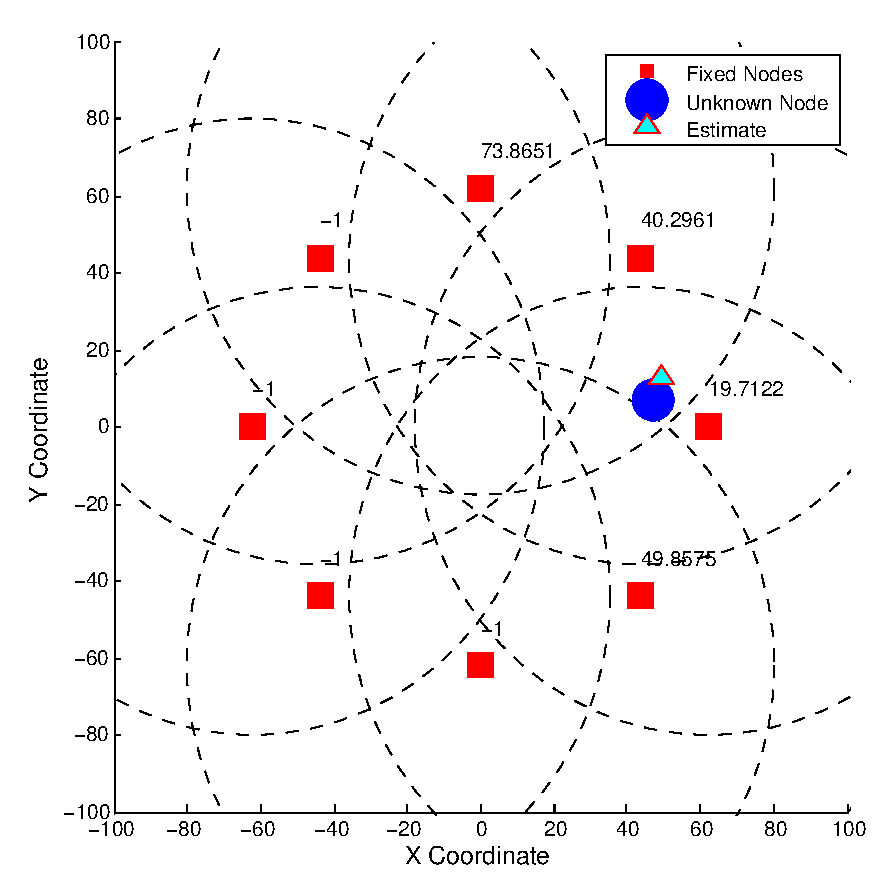
\includegraphics[width=0.5\textwidth]{figures/localization_snapshot2}
\caption{\label{fig:loc_overview}Multi-agent localization application: the square nodes with known location attempt to localize the unknown circle node through consensus. }
\end{figure}


Oftentimes a system is composed of multiple nodes connected by either wired or wireless communication.  As an example, consider a network of 8 nodes with wireless radio capabilities.  Each node is capable of sensing a noisy measurement that corresponds roughly to the distance of some unknown object to the node, whose location is known.  For example, these nodes could be taking audio measurements and inferring the distance of a vehicle traveling around a track.  From these distance measurements, we would like to estimate the $(x,y)$ coordinate of the unknown vehicle.  This system is illustrated in Figure \ref{fig:loc_overview}, where the unknown object makes a counter-clockwise path and the known sensor nodes take noisy measurements if the object is within their radius of observation, shown with dashed circles.  Here the unknown object is traveling on a track of 300 m circumference at the speed of 0.4 km/h. The 8 known nodes can `observe' a linear distance to the unknown node if it is within 80 m.  Each node operates two tasks: (1) a radio with a variable frequency transmission, and (2) a sensor that samples a variable number of points and averages the samples.   Allowing the radio more active time will reduce the latency in reported estimates of the unknown node, while allowing the sensing task more time will generate more reliable estimates.  The task priorities $p_i$ along with the tool described in Section \ref{sec:vartos:tool} would help a developer give preference to one or the other. For the sake of our comparison, we keep the priorities the same and choose knob ranges to allow the sensor to average between 1 and 100 samples and to allow the radio to transmit anywhere from 10 Hz to 0.1 Hz.  Because these peripherals are simulated, each task has been padded with NOP instructions in order to simulate work that an actual system might be doing.  If we look at a 1000 minute time slice of the estimation process as shown in Figures \ref{fig:loc_error_var} and \ref{fig:loc_error_novar}, we see that the variance of the estimation error is much greater if we assume worst-case power and thus average fewer samples and much less if we use VaRTOS with instance-specific power models.  When many samples are averaged, the noise is reduced and each estimate is the result of consensus between more reliable measurements.  In other words, for the same lifetime specifications, the system using VaRTOS greatly outperforms the system that assumes worst-case power consumption.  While the deployment assuming worst-case consumption suffers from an average error variance of 59.7, the VaRTOS deployment has an average error variance of only 26.9, a 54.9\% improvement.  The periodic nature of the high variance peaks in estimation error for both Figures \ref{fig:loc_error_var} and \ref{fig:loc_error_novar} can be attributed to the circular nature of the application setup (Figure \ref{fig:loc_overview}).  When the unknown object comes within view of nodes with less reliable measurements, the estimation error is much poorer. 

\begin{figure*}[t]
\centering
{\centering
\begin{minipage}{0.47\textwidth}
  \centering
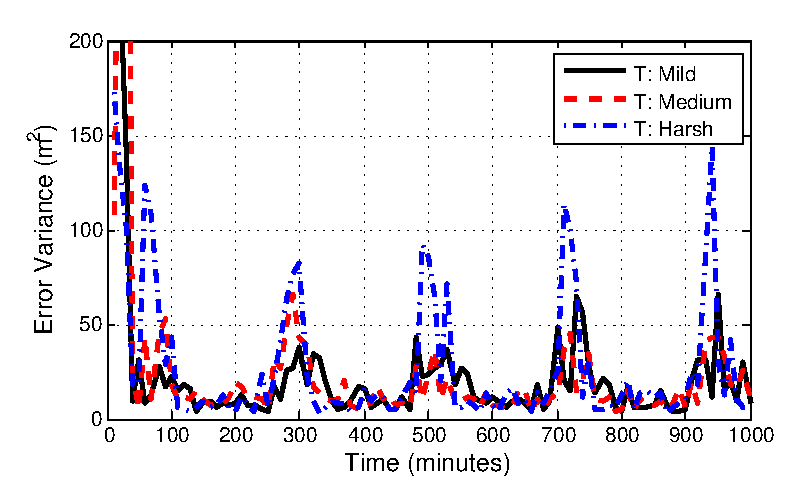
\includegraphics[width=\textwidth]{figures/localization_variance_var}
  \captionof{figure}{\label{fig:loc_error_var}Reduced error variance for multi-agent localization using instance power modeling with VaRTOS}
\end{minipage}
\hspace{.04\textwidth}
\begin{minipage}{0.47\textwidth}
  \centering
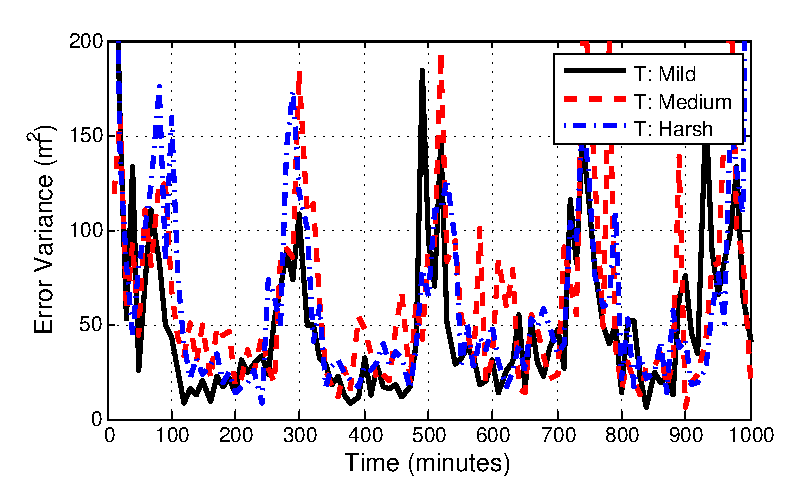
\includegraphics[width=\textwidth]{figures/localization_variance_novar}
  \captionof{figure}{\label{fig:loc_error_novar}Increased error variance for multi-agent localization assuming worst-case power }
\end{minipage}
}
\end{figure*}



Furthermore, the reduction in error variance when using VaRTOS does not come at the price of increased radio latency; the radio latency on the average will improve by using VaRTOS as well, as shown  for the case of harsh temperature profiles in the resulting optimal task performance in Table \ref{tab:loc_knobs}. The errors in energy consumption for this application are equivalent to those shown in Figure \ref{fig:app1_energy}, and thus we omit them here for the sake of brevity.


\begin{table}
\caption{\label{tab:loc_knobs}Task performance for multi-agent localization with and without VaRTOS with a harsh temperature profile}
\centering
\begin{tabular}{r|cccccccc}
\hline
Node ID & \#1 & \#2 & \#3 & \#4 & \#5 & \#6 & \#7 & \#8 \\ \hline
VaRTOS \# Avgs. & 35 & 34 & 31 & 30 & 28 & 27 & 23 & 10 \\
WC \# Avgs. & 6 & 6 & 6 & 6 & 6 & 6 & 6 & 6 \\
VaRTOS Freq (Hz) & 1.798  & 1.719 & 1.583 &1.527 & 1.459 & 1.380 & 1.176  & 0.525 \\
WC Freq (Hz) & 0.287 & 0.287 & 0.287 & 0.287 & 0.287 & 0.287 & 0.287 & 0.287 \\ \hline
\end{tabular}
\end{table}


%\begin{figure}
%\centering
%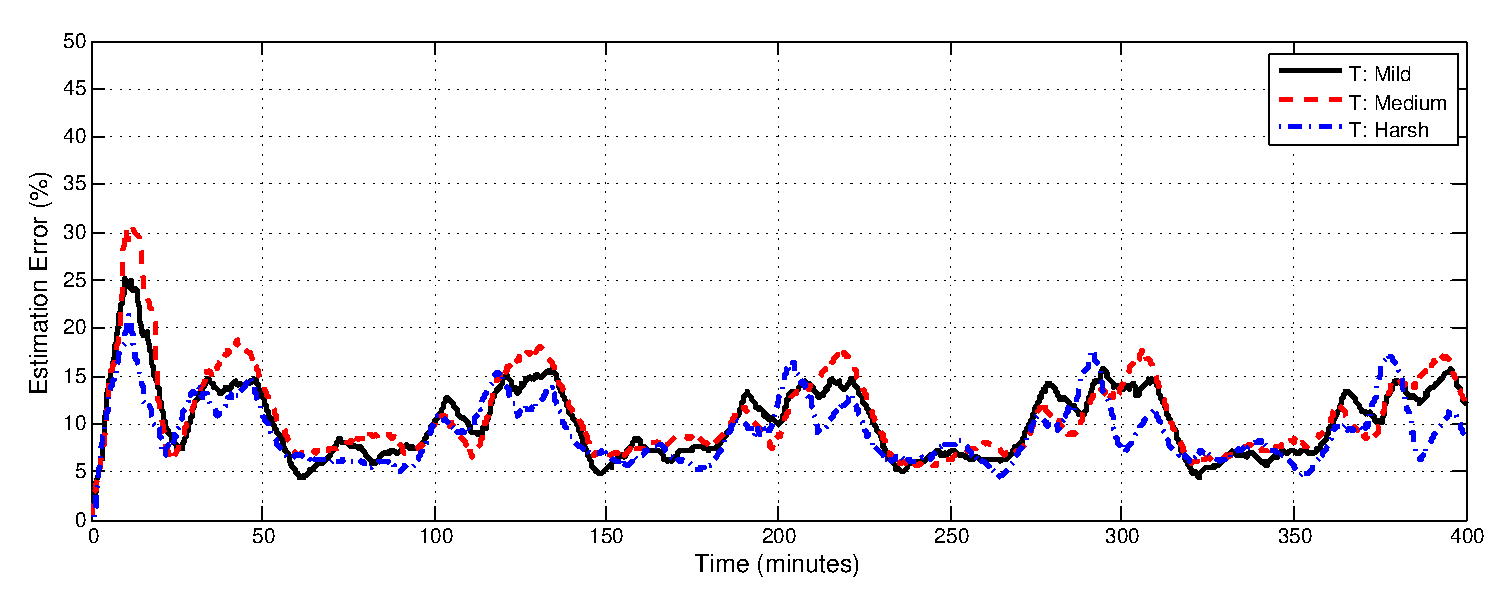
\includegraphics[width=0.5\textwidth]{figures/localization_var.eps}
%\caption{\label{fig:app1}App 1 dutycycle comparison}
%\end{figure}
%
%\begin{figure}
%\centering
%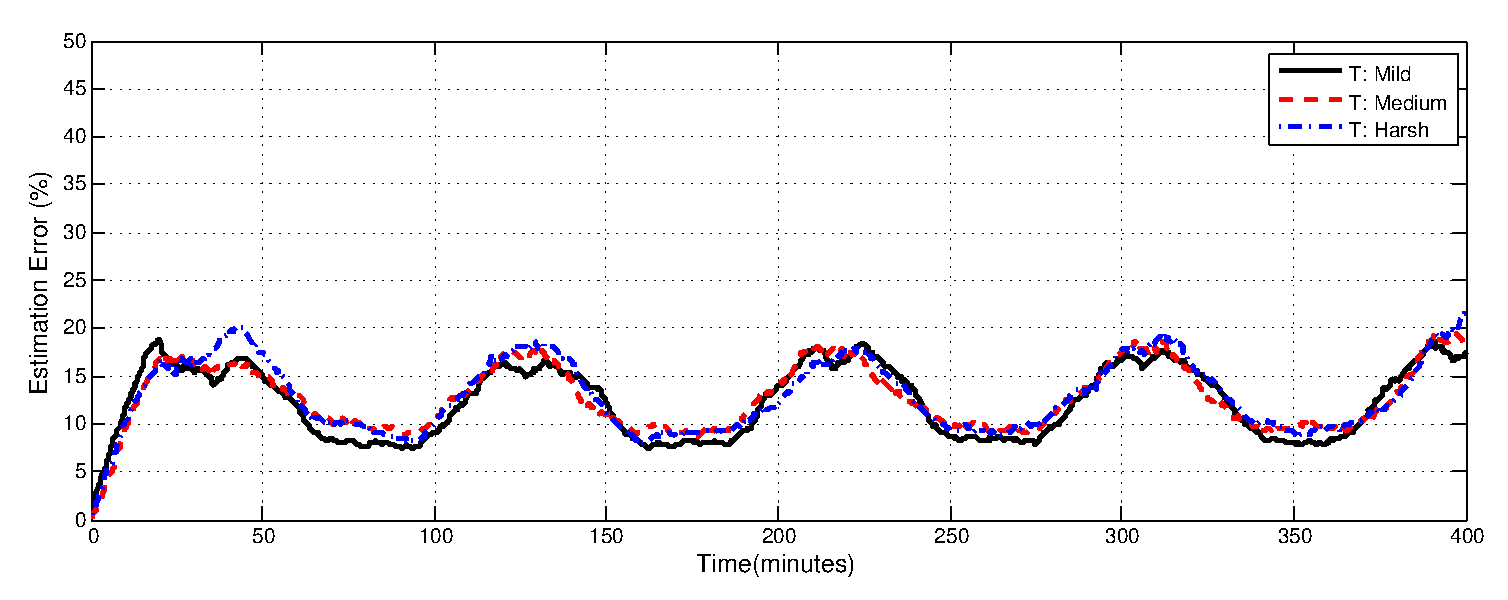
\includegraphics[width=0.5\textwidth]{figures/localization_novar.eps}
%\caption{\label{fig:app1}App 1 dutycycle comparison}
%\end{figure}
%

%\begin{figure}
%\centering
%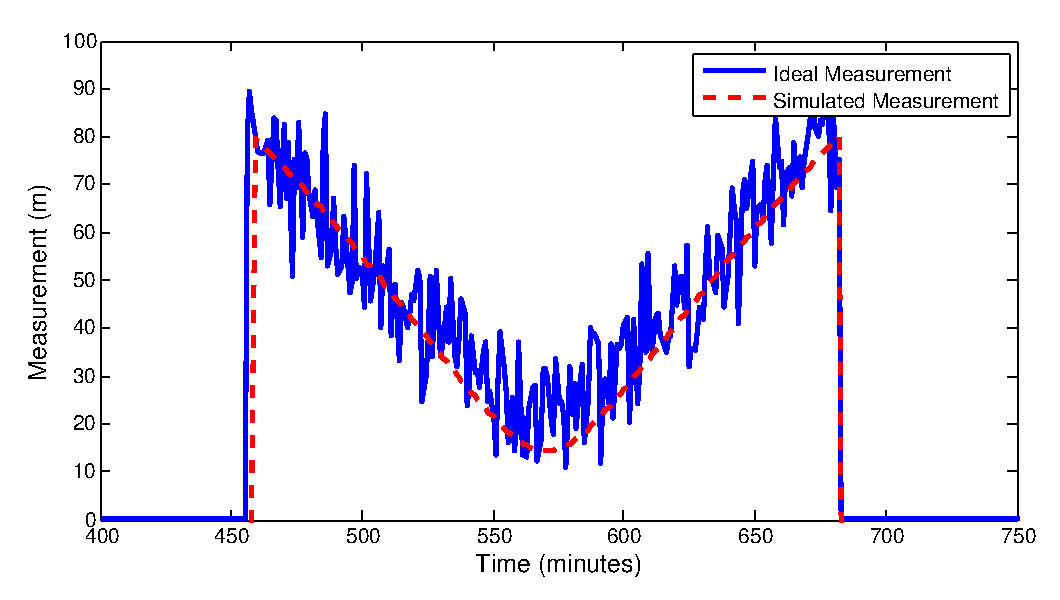
\includegraphics[width=0.5\textwidth]{figures/localization_stream_wc.eps}
%\caption{\label{fig:app1}App 1 dutycycle comparison}
%\end{figure}
%
%\begin{figure}
%\centering
%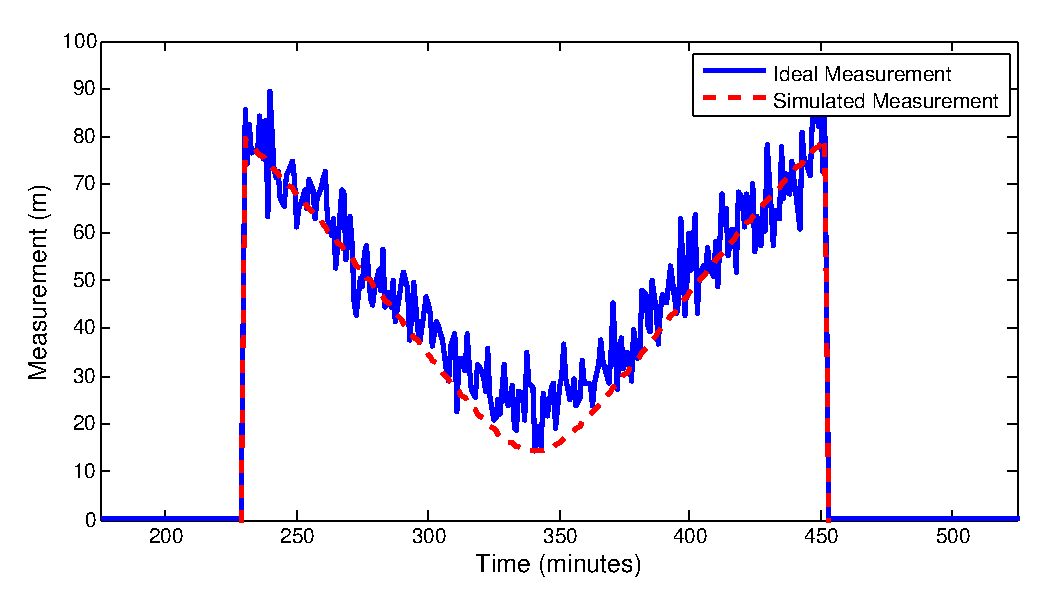
\includegraphics[width=0.5\textwidth]{figures/localization_stream_bc.eps}
%\caption{\label{fig:app1}App 1 dutycycle comparison}
%\end{figure}
%
%\begin{figure}
%\centering
%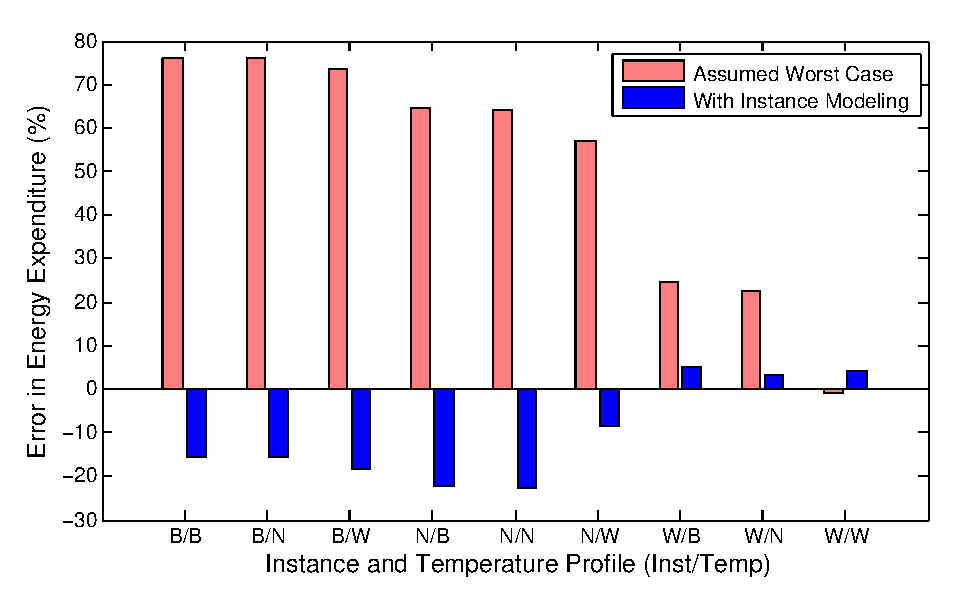
\includegraphics[width=0.5\textwidth]{figures/app3_energycomp.eps}
%\caption{\label{fig:app1}App 1 dutycycle comparison}
%\end{figure}



\subsection{Prediction-type Applications}
We now move away from wireless sensor network applications and look at systems of just a single node.  In particular, we consider an application where we would like to predict one quantity from another correlated but noisy quantity: in our case, we will predict velocity from position, perhaps again on a vehicle of some kind.  Here our tool of choice will be the Kalman filter, as it has become such a widely used tool even for resource-constrained applications. We are interested in calculating an estimate $\hat{v}$ of the velocity $v$ from measurements of the position, $y$, at various frequencies controlled again by a knob.  The system evolves according to the simple state space recursion: 

$$x_{k+1} = A_kx_k + B_ku_k~; ~~~~~ y_k = C_kx_k~;~~~~A_k= \begin{bmatrix}1 & \Delta t \\ 0 & 1\end{bmatrix}~~~~B_k = \begin{bmatrix} 0 & 1 \end{bmatrix}~~~~C_k = \begin{bmatrix} 1 & 0 \end{bmatrix}$$

For our case, $u_k$ will be a sinusoidal velocity input, and the goal is for $\hat{v}$ to track this input.  Intuitively, a faster sample rate for $y_k$ (meaning $\Delta t$ changes in $A$ as well) should give more accurate predictions of $\hat{v}$, because it is easier to predict states within the near future than it is to predict them in the distant future.  The Kalman recursion itself is omitted here, but we note that the Kalman gain and error covariance matrices (commonly denoted $K_{p,k}$ and $P_{k+1|k}$, respectively)  have to be modified on a per-instance basis in order to accommodate the varying sampling period, $\Delta t$. 


\begin{figure*}[t]
\centering
{\centering
\begin{minipage}{0.47\textwidth}
  \centering
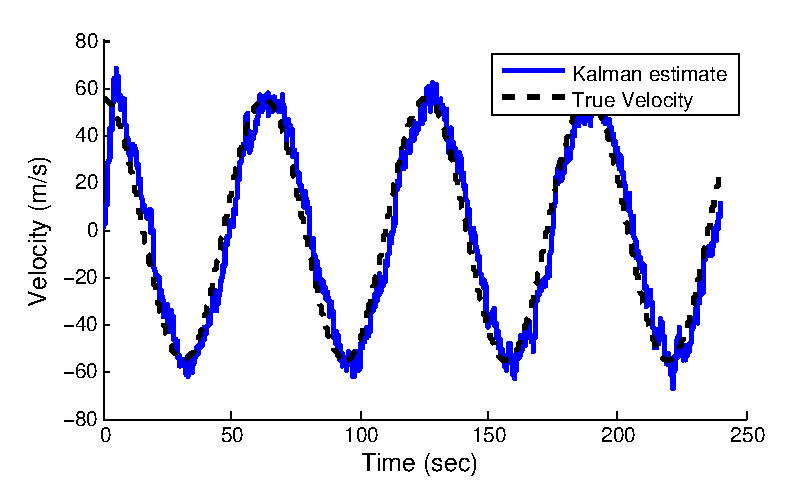
\includegraphics[width=\textwidth]{figures/kalman_example_vel}
  \captionof{figure}{\label{fig:kalman_ex}Kalman filter prediction of velocity from noisy position measurements}
\end{minipage}
\hspace{.04\textwidth}
\begin{minipage}{0.47\textwidth}
  \centering
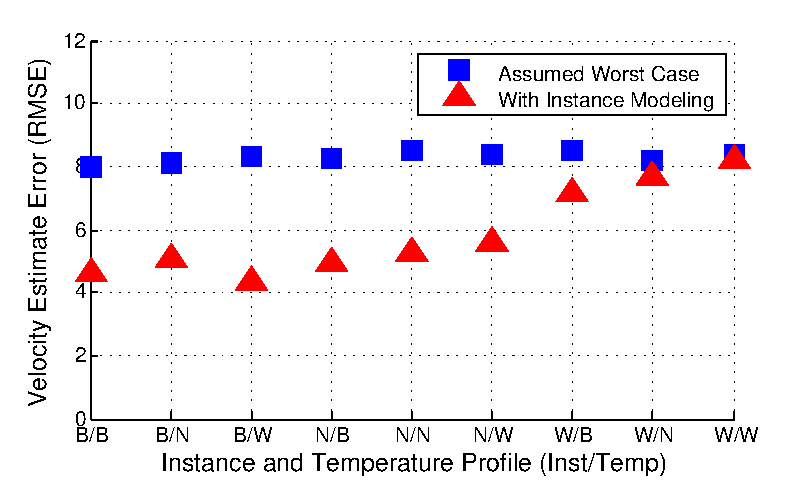
\includegraphics[width=\textwidth]{figures/kalman_results}
  \captionof{figure}{\label{fig:kalman_errors}Error (RMSE) in Kalman predictions when assuming worst case power consumption and when using VaRTOS }
\end{minipage}
}
\end{figure*}



Figure \ref{fig:kalman_ex} shows an example of the velocity input, $u_k$, as well as the estimated velocity as calculated by the Kalman filter on position $y_k$. Here the position readings are subjected to additive white Gaussian noise $\sim \normal(0, 50~m)$, and likewise the Kalman estimation of velocity contains some noise as well.  If we allow $\Delta t$ to assume values within the range $\Delta t \in [0.1~\text{s}, 10~\text{s}]$ by letting our knob vary as before, the quality of the estimate $\hat{v}$ will increase or decrease in accordance with energy surpluses and deficits, respectively.  Figure \ref{fig:kalman_errors} shows the error (RMSE) in estimating the velocity from noisy position measurements for systems assuming worst-case power and for those using instance-specific modeling with VaRTOS.  As before, the $x$-axis represents combinations of power instances (best-, nominal-, and worst-case) as well as temperature profiles (mild/best, medium/nominal, and harsh/worst). While the worst-case system has a constant error across all combinations, the VaRTOS results show a reduction in prediction error when additional work can be performed without sacrificing lifetime (i.e. those cases where weather and power instance result in a reduction in energy consumption over the worst-case). This improvement can be as much as 42.5\% in many cases. 


%
%\begin{figure}
%\centering
%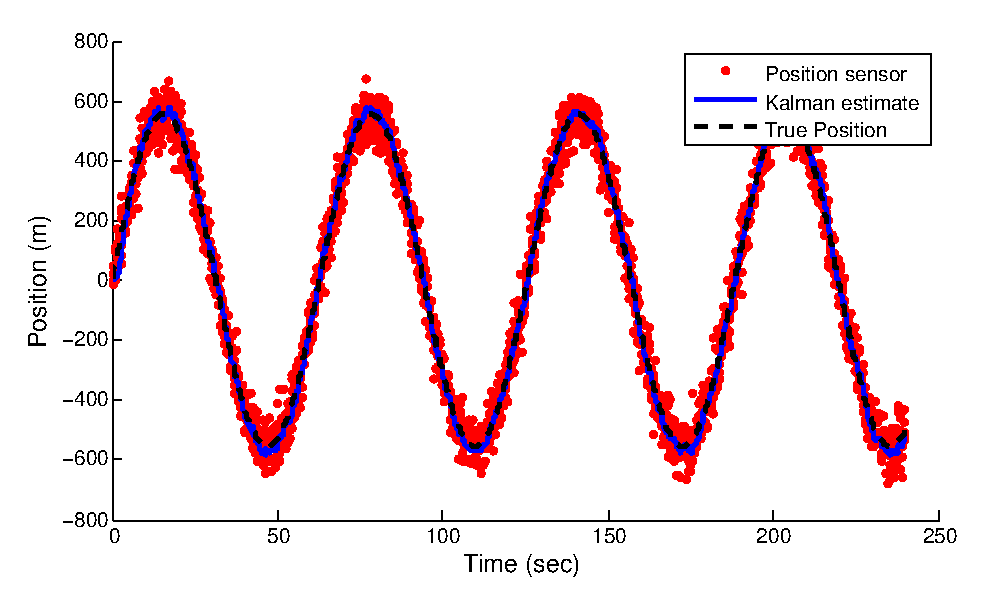
\includegraphics[width=0.5\textwidth]{figures/kalman_example_pos.eps}
%\caption{\label{fig:app1}App 1 dutycycle comparison}
%\end{figure}


\subsection{Block Processing Applications}

In some cases, a developer may have a number of signal processing (or similar) routines that would help to clean up or extract data from a particular signal.  In most cases, the total number of potential sensor processing blocks is likely to be small, and more importantly it is unlikely that each of these blocks will take the same time and thus the same power to complete.  In other words, the functions $\mathcal{K}_i$ that map knob values into duty cycles are no longer a very good fit, as the curve $k_i\rightarrow d_i$ is no longer linear.  As an example, consider a system with two sensor streams, each with 5 potential sensing blocks that all increase the quality of the application as a whole.  These tasks each take a distinct number of computer cycles to complete, as summarized in Table \ref{tab:blocks}.
\begin{table}
\caption{\label{tab:blocks}Processor cycle counts for a multi-block signal processing application}
\centering
\begin{tabular}{r|ccccc}
\hline
Block \# & 1 & 2 & 3 & 4 & 5 \\ \hline
Sensor 1 Block Cycles & 20000 & 5000 & 10000 & 25000 & 6000 \\
Sensor 2 Block Cycles & 14000 & 9000 & 15000 & 24000 & 8000 \\ \hline
\end{tabular}
\end{table}

%\begin{table}
%\caption{\label{tab:block_knobs}Optimal knob values (\# of blocks executed) for a multi-block signal processing application}
%\centering
%\begin{tabular}{r|ccccc}
%\hline
%Temperature & Power  & Sensor 1 & Sensor 1 & Sensor 2 & Sensor 2  \\
%& Instance & Worst-Case & VaRTOS & Worst-Case & VaRTOS \\ \hline
%Mild Weather & BC & 1 & 4 & 0 & 5\\
% & NC & 1 & 4  & 0 & 5\\
%& WC & 1 & 4  & 0 & 5\\
%Medium Weather & BC & 1 & 4  & 0 & 4\\
% & NC & 1 & 4  & 0 & 4\\
% & WC & 1 & 3  & 0 & 4\\
%Harsh Weather & BC & 1 & 1  & 0 & 2\\
% & NC & 1 & 1  & 0 & 2\\
% & WC & 1 & 0  & 0 & 1\\ \hline
%\end{tabular}
%\end{table}

\begin{figure}
\centering
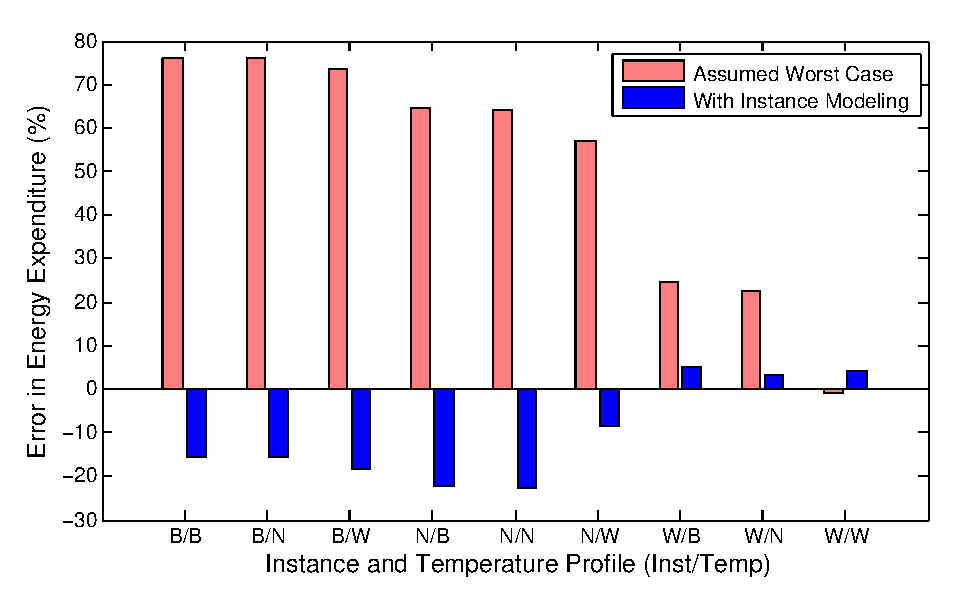
\includegraphics[width=0.6\textwidth]{figures/app3_energycomp}
\caption{\label{fig:app3_energycomp}Energy consumption errors for a mult-block signal processing application }
\end{figure}

The cycles  here have been arbitrarily chosen in part to show how VaRTOS responds to violations in architecture assumptions (linearity and granularity of task knobs).  If we try to schedule these two tasks using VaRTOS with $E = 12960~J$ and $L = 8760~h$ as before, the resulting errors in energy consumption will be those shown in Figure \ref{fig:app3_energycomp}.  In this case, the number of blocks executed using VaRTOS is on average 2.8 for sensor 1 and 3.5 for sensor 2 while worst-case power assumption resulted in 1 block between both sensors combined. In other words, while VaRTOS gives over a 64\% signal processing improvement in this application, the errors in energy expenditure are on average much larger than the errors shown in Figure \ref{fig:app1_energy}; indeed they would be even larger had our cycle counts shown in Table \ref{tab:blocks} varied even more or had the number of blocks been even fewer than 5.  While VaRTOS can help reduce energy errors to some extent in applications similar to this multi-block signal processing example, care should be taken to ensure that the assumptions made in Section \ref{sec:optimization} are not completely ignored. 





